\chapter{Results}
\label{ch:results}

This chapter reports every result on the held-out test split, scored once, with
selection done on validation only (Section~\ref{sec:protocol}). It begins with a
correction to results reported in earlier drafts, because every later number depends
on it, and then answers the five research questions in turn.

\section{A Correction: Two Problems in the Earlier Results}
\label{sec:leak}

Earlier drafts of this work (Chapter~\ref{ch:method}, version~1) reported an ensemble
reaching $0.865$ on real test charts. That number had two problems.

\paragraph{Selection on the test set.} The ensemble was chosen by ranking every
combination of trained models on test accuracy. Selecting the same models on
validation instead gives $0.845$. The difference is small, but a number chosen on the
test set is not a test result.

\paragraph{A rendering leak.} Version-1 time-series charts carried marks that depended
on the label (Section~\ref{sec:v2}). To measure how much the models relied on them, the
same 1{,}000 test time series were rendered twice with identical styles, once with the
marks and once without, and scored with two ResNets trained on version 1
(Table~\ref{tab:leak}, Figure~\ref{fig:leak}).

\begin{table}[h]\centering\small
\caption{Accuracy of version-1 models on test time series rendered with and without the
label-dependent marks. Only the marks differ between the two renders.}
\label{tab:leak}
\begin{tabular}{lcccc}
\toprule
& \multicolumn{2}{c}{\textbf{ResNet-101}} & \multicolumn{2}{c}{\textbf{ResNet-50}} \\
\cmidrule(lr){2-3}\cmidrule(lr){4-5}
\textbf{Test charts} & with marks & without & with marks & without \\
\midrule
Real time series ($n=305$)       & 0.957 & \textbf{0.311} & 0.944 & \textbf{0.407} \\
Synthetic time series ($n=695$)  & 1.000 & 0.801 & 1.000 & 0.911 \\
\quad level shift                & 1.000 & 0.355 & 1.000 & 0.705 \\
\quad increasing                 & 0.975 & 0.570 & 0.930 & 0.570 \\
\quad seasonal (never marked)    & 0.970 & 0.970 & 0.990 & 0.990 \\
\bottomrule
\end{tabular}
\end{table}

\begin{figure}[h]\centering
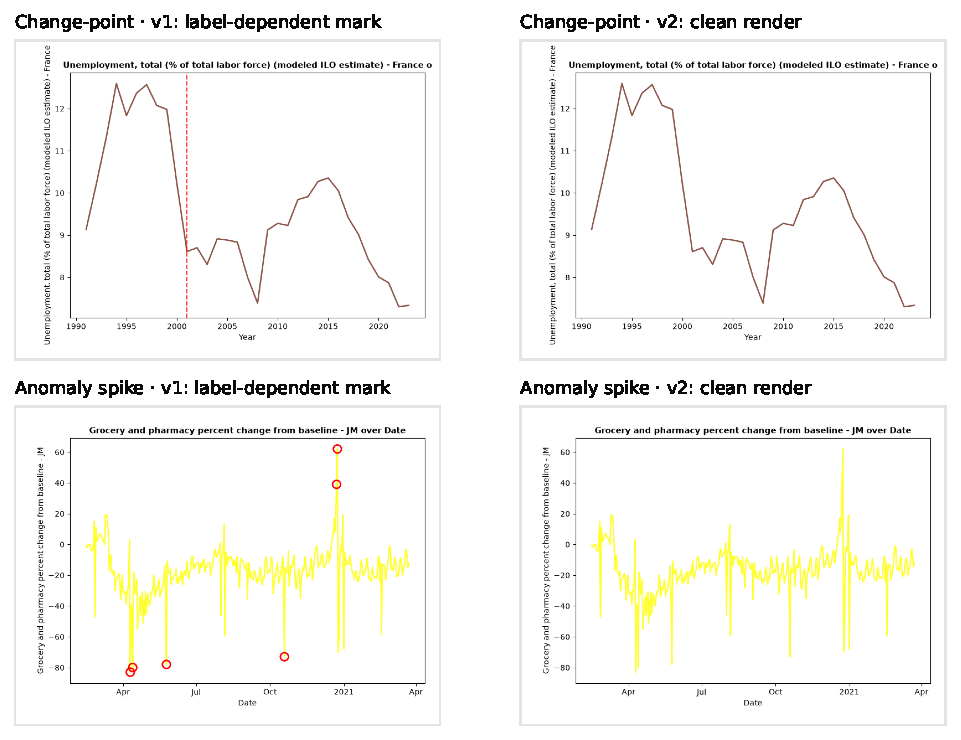
\includegraphics[width=\linewidth]{fig_marks_examples.pdf}\\[0.5em]
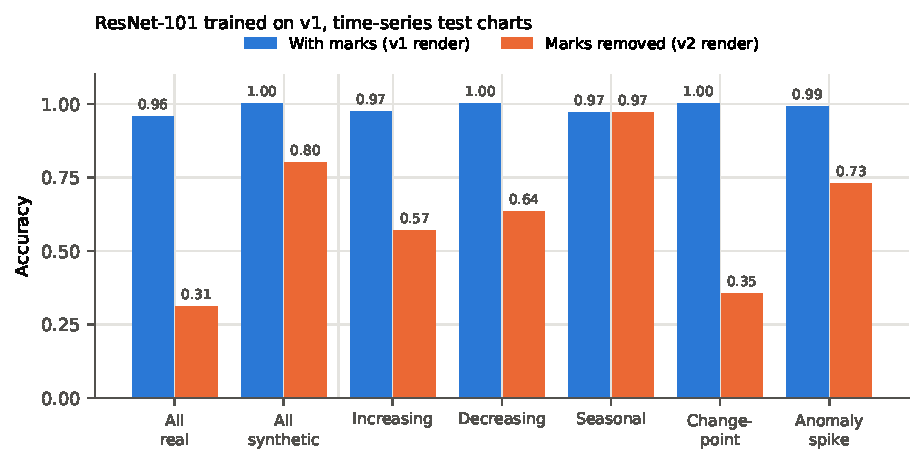
\includegraphics[width=\linewidth]{fig_marks_ablation.pdf}
\caption{Top: the same real data rendered with a version-1 label-dependent mark and in
the released version-2 form. Bottom: accuracy of a version-1 ResNet-101 with and
without the marks.}
\label{fig:leak}
\end{figure}

Without the marks, accuracy on real time series fell from $0.957$ to $0.311$: the
models had largely learned to read the annotation rather than the data. The seasonal
class, the only temporal class that never carried a mark, was unaffected, which isolates
the cause. The zero-shot vision--language models of Section~\ref{sec:rq1}, which never
saw version-1 training data, changed by only 1--2.5 points on all real charts and
4--10 points on real time series. This is shortcut learning~\citep{geirhos} of the
plainest kind, and the shortcut audit (Table~\ref{tab:bias}) did not detect it, because
the audit examines metadata and pixel statistics rather than what a trained model
relies on.

\textbf{Every result from here on uses version 2, trains new models on it, and selects
on validation only.}

\section{RQ1: Can a Model Identify the Finding from the Chart Alone?}
\label{sec:rq1}

Table~\ref{tab:main} gives the main results and Figure~\ref{fig:main} the comparison.
The deployed ensemble (the equal-weight average of the two full-recipe models) reaches
\textbf{0.867} on the 1{,}192 real test charts (95\% CI $[0.846, 0.886]$) and
\textbf{0.999} on synthetic ones, $0.959$ over all 4{,}000 test charts. Macro-F1 on
real charts is $0.776$, lower than accuracy because the rarest real classes are also
the hardest.

\begin{table}[h]\centering\small
\caption{Accuracy on the 1{,}192 real test charts drawn by three plotting libraries,
and on synthetic test charts. Brackets: 95\% bootstrap CI. $^\dagger$Fixed 400-chart
synthetic sample.}
\label{tab:main}
\resizebox{\linewidth}{!}{%
\begin{tabular}{lcccc}
\toprule
 & \multicolumn{3}{c}{\textbf{Real test charts}} & \\
\cmidrule(lr){2-4}
\textbf{System} & \textbf{matplotlib} & \textbf{Plotly} & \textbf{Vega-Lite} & \textbf{Synthetic} \\
\midrule
Chart-type prior (no pixels)            & \multicolumn{4}{c}{0.288 (all test charts)} \\
Qwen2.5-VL-3B, zero-shot                & 0.306 [0.281, 0.332] & -- & -- & 0.303$^\dagger$ \\
Qwen2.5-VL-7B, zero-shot                & 0.411 [0.383, 0.440] & -- & -- & 0.498$^\dagger$ \\
Qwen3-VL-8B, zero-shot                  & 0.468 [0.439, 0.496] & -- & -- & 0.648$^\dagger$ \\
\midrule
ResNet-101, balanced split              & 0.841 & 0.747 & 0.607 & 0.997 \\
ResNet-50, balanced split               & 0.828 & 0.722 & 0.608 & 0.998 \\
ResNet-101, + supplementary pool        & 0.840 & 0.735 & 0.602 & 0.999 \\
ResNet-50, + supplementary pool         & 0.845 & 0.760 & 0.599 & 0.998 \\
DenseNet-121, + supplementary pool      & 0.861 & 0.771 & 0.638 & 0.997 \\
ResNet-101, + pool + renderer aug.      & 0.859 & 0.854 & 0.650 & 0.998 \\
DenseNet-121, + pool + renderer aug.    & 0.855 & 0.852 & 0.712 & 0.998 \\
\textbf{Ensemble (two full-recipe models)} & \textbf{0.867} [0.846, 0.886] & \textbf{0.857} [0.836, 0.877] & \textbf{0.716} [0.690, 0.741] & \textbf{0.999} \\
\midrule
Statistical oracle on the data table    & \multicolumn{4}{c}{0.9995 (all test charts)} \\
\bottomrule
\end{tabular}}
\end{table}

\begin{figure}[h]\centering
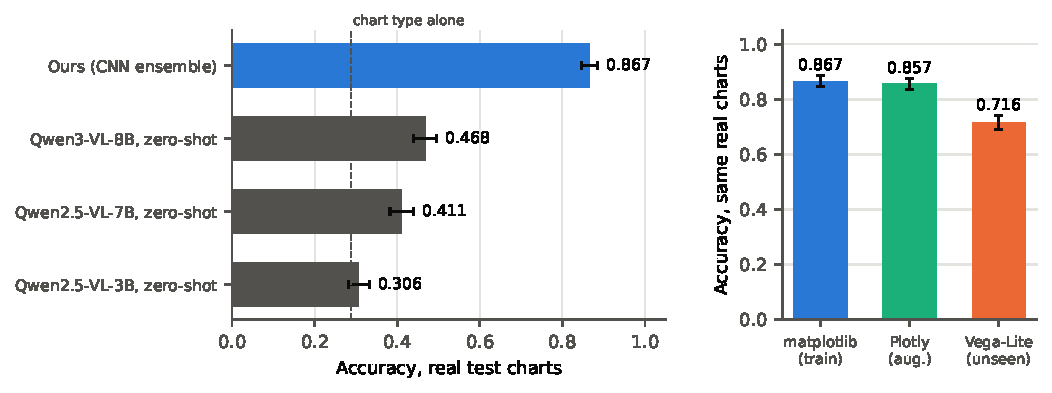
\includegraphics[width=\linewidth]{fig_results.pdf}
\caption{Left: accuracy on the real test charts (matplotlib renders) with 95\% bootstrap
CIs; the dashed line is the chart-type prior. Right: the deployed ensemble on the same
real charts drawn by the training renderer, by Plotly (used only as training
augmentation) and by Vega-Lite (never seen).}
\label{fig:main}
\end{figure}

\paragraph{Zero-shot vision--language models cannot do this task reliably.} The best,
Qwen3-VL-8B, reaches 0.468; the smallest, Qwen2.5-VL-3B, is barely above the 0.288
floor that uses no pixels at all. The ensemble is right on 511 charts where Qwen3-VL-8B
is wrong and wrong on only 36 where it is right (exact McNemar $p<10^{-100}$; the same
holds for the other two models). Naming a statistical finding from a chart is therefore
not a capability current general-purpose VLMs already have.

\paragraph{How the result was built.} Each step in Table~\ref{tab:main} changes one
thing. Adding the supplementary real pool helped ResNet-50 (+1.7 points) but not
ResNet-101 ($-0.1$); DenseNet-121 trained on the pool was the strongest single model on
matplotlib charts ($0.861$). Renderer augmentation raised ResNet-101 from $0.840$ to
$0.859$ and, as the next section shows, mattered far more on other renderers. Choosing
the ensemble differently changes little: averaging all seven trained models gives
$0.862$, greedy selection on validation $0.865$.

\paragraph{Where the model fails.} Figures~\ref{fig:conf} and~\ref{fig:perclass} break
the result down. Errors stay almost entirely within a family, and the family with the
most errors is distribution shape ($0.763$ on real charts, against $0.886$--$0.930$ for
the others). The commonest confusions are between classes that differ in degree rather
than kind: bimodal read as right-skewed (19 of 100), heavy-tailed read as right-skewed
(13 of 26) and significant group differences read as none (12 of 100). Accuracy is
lowest where real examples are rare: heavy tails ($0.385$, $n=26$), seasonality
($0.462$, $n=13$), left skew ($0.474$, $n=19$), and the inverted-U relationship, of
which only two real test charts exist.

\begin{figure}[h]\centering
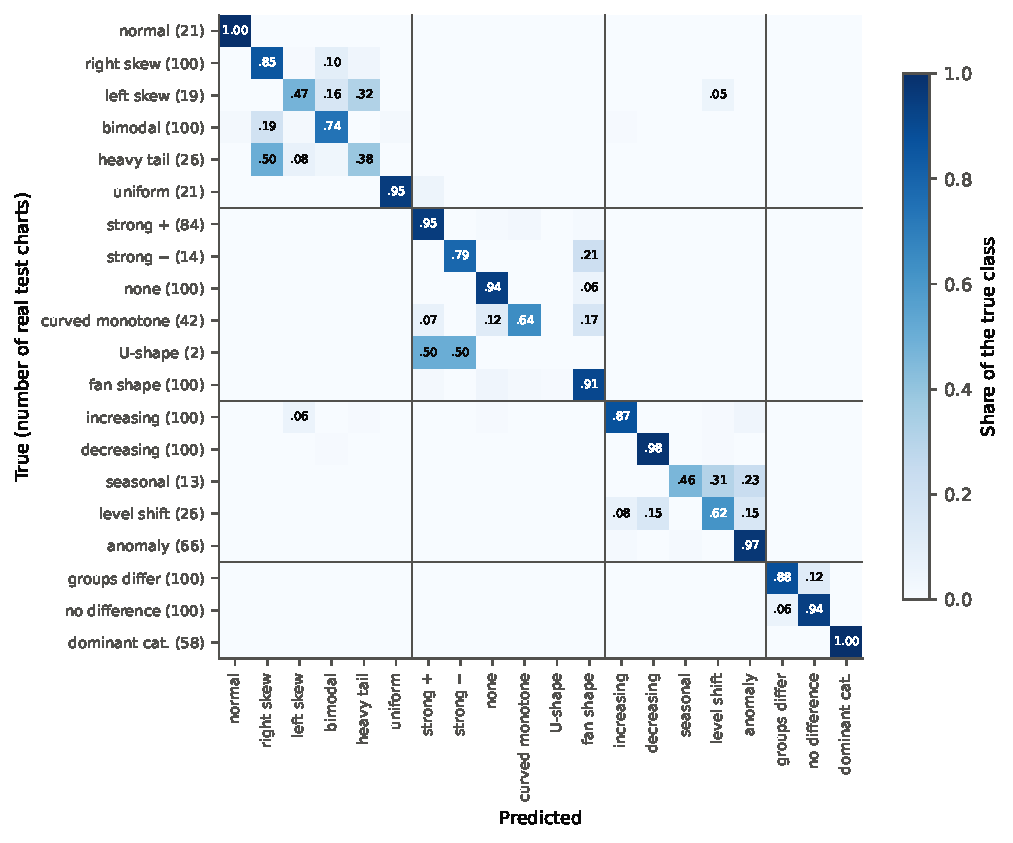
\includegraphics[width=0.92\linewidth]{fig_confusion.pdf}
\caption{Confusion matrix of the deployed ensemble on the 1{,}192 real test charts,
normalised by true class; lines separate the four families. The number of real charts
per class is in brackets.}
\label{fig:conf}
\end{figure}

\begin{figure}[h]\centering
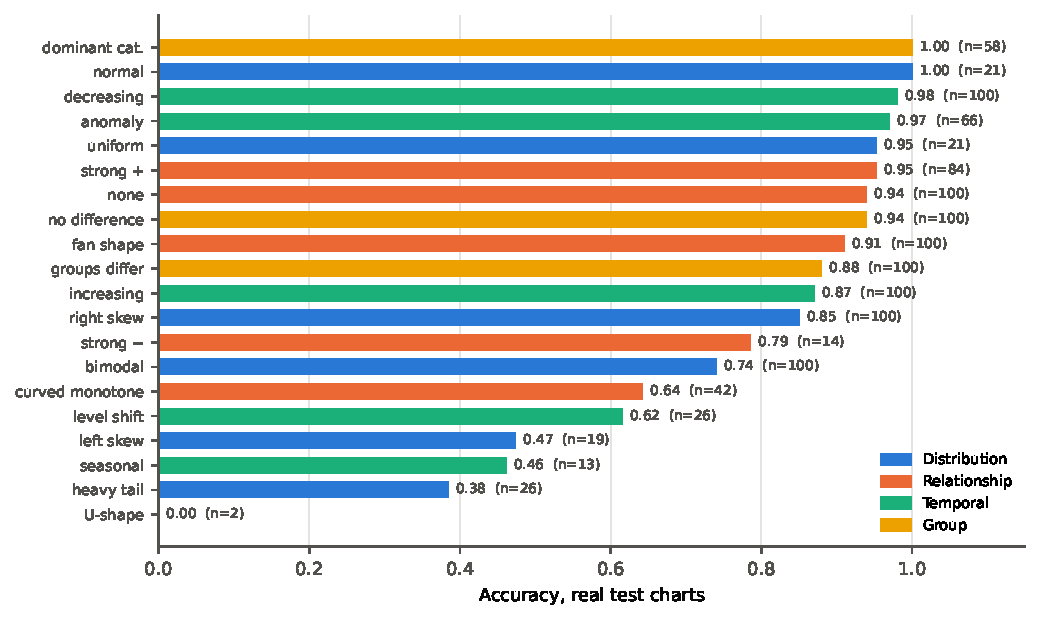
\includegraphics[width=\linewidth]{fig_per_class.pdf}
\caption{Accuracy of the deployed ensemble per class on the real test charts.}
\label{fig:perclass}
\end{figure}

\paragraph{Answer to RQ1.} Yes, for most findings. A fine-tuned vision model names the
statistical finding of a real chart correctly 86.7\% of the time without being asked a
question, far above both the pixel-free floor and current zero-shot VLMs. It remains
unreliable for subtle distribution shapes and for classes with little real data.

\section{RQ2: Model Insights versus a Deterministic Statistical Pipeline}
\label{sec:rq2}

The deterministic pipeline is the verification battery run on the chart's stored data
table. It recovers the finding for 0.9995 of test charts, and the two exceptions lie
within 1\% of a guard threshold and fall to \emph{no class} rather than to a wrong one.
Its numbers are exact by construction.

The generative model (Qwen2-VL-2B with QLoRA, Section~\ref{sec:models}) was evaluated on
a 300-chart test subset. It named the correct finding for $0.800$ of charts ($0.683$ on
real, $0.844$ on synthetic), but \textbf{only 13.8\% of the numbers it cited matched the
ground-truth statistics}. It has learned the vocabulary and structure of statistical
reasoning while largely inventing the supporting numbers. This model was trained and
scored on version-1 renders; its class accuracy on time series may be inflated by the
leak, but numeric fidelity concerns the numbers in its text and is not affected by marks.

\paragraph{Answer to RQ2.} Far below. The rule-based pipeline is essentially always right
and exact; the generative model is right about the finding four times in five but cites
correct numbers about one time in seven. Fluent statistical language is much easier to
produce than true statistical language, and only a dataset with verified statistics can
tell them apart.

\section{RQ3: Is the Model Looking at the Evidence?}
\label{sec:rq3}

We tested whether the deployed models attend to the evidence that licenses a label,
using the pointing game of Section~\ref{sec:models}: for each of the 1{,}023 real test
charts that carry at least one evidence box, a hit is a Grad-CAM peak inside an evidence
box, and the control is a random point in the plot area (Table~\ref{tab:grounding}).

\begin{table}[h]\centering\small
\caption{Pointing game on 1{,}023 real test charts. \emph{Gain} is the pointing rate
minus the random-point control, with a 95\% bootstrap CI.}
\label{tab:grounding}
\begin{tabular}{lccc}
\toprule
\textbf{Charts} & \textbf{Pointing} & \textbf{Random control} & \textbf{Gain [95\% CI]} \\
\midrule
Temporal ($n=305$)      & 0.649 & 0.495 & $+0.154$ [$+0.139$, $+0.168$] \\
Group ($n=258$)         & 0.599 & 0.489 & $+0.110$ [$+0.064$, $+0.153$] \\
Relationship ($n=173$)  & 0.642 & 0.569 & $+0.073$ [$+0.029$, $+0.115$] \\
Distribution ($n=287$)  & 0.253 & 0.254 & $-0.002$ [$-0.035$, $+0.033$] \\
\midrule
ResNet-101 member       & 0.543 & 0.439 & $+0.105$ [$+0.081$, $+0.130$] \\
DenseNet-121 member     & 0.504 & 0.439 & $+0.066$ [$+0.042$, $+0.089$] \\
\textbf{All}            & \textbf{0.524} & \textbf{0.439} & $\mathbf{+0.085}$ [$+0.068$, $+0.102$] \\
\bottomrule
\end{tabular}
\end{table}

The models point at the evidence more often than chance overall ($+8.5$ points), most
clearly for time series ($+15.4$) and group comparisons ($+11.0$), less for relationships
($+7.3$), and \emph{not at all} for distributions ($-0.2$, CI spanning zero). Pointing is
slightly better when the prediction is correct (0.570 and 0.533 for the two members).

Two readings are possible for the distribution family, and the data cannot yet separate
them. A distribution's shape is a property of the whole histogram or density rather than
of one region, so an evidence box around the modal bin or the outlier band may simply be
the wrong reference for where a model should look. Alternatively, the models may judge
shape from global cues. Either way, distribution is also the family with the lowest
accuracy (0.763), so weak grounding and weak accuracy coincide.

\paragraph{Answer to RQ3.} Partly. The model's attention is tied to the verified evidence
beyond chance for three of four families, but only modestly: about half of all peaks fall
inside an evidence box, against 44\% for a random point. The CNN classifiers are not
generating insights, so this measures whether their decisions rest on the evidence, not
whether a generated sentence is traceable; the generative model's traceability is limited
by its 13.8\% numeric fidelity (Section~\ref{sec:rq2}).

\section{RQ4: Generalisation to Real-World Charts}
\label{sec:rq4}

Real-world generalisation has two parts: real \emph{data}, and charts drawn by
\emph{other tools}.

\paragraph{Real data.} On matplotlib charts the gap between synthetic and real test
charts is 13.2 points ($0.999$ against $0.867$). Real charts are harder: 44\% of real
samples fall in the hardest evidence-margin tertile against 29\% of synthetic ones, and
real data are noisier and less clean-cut than generated data.

\paragraph{Other plotting libraries.} Trained on matplotlib alone, every model loses
8.5--10.6 points when the same real data is drawn by Plotly and 22--25 points when it
is drawn by Vega-Lite (Table~\ref{tab:main}). The models had learned part of matplotlib's
appearance. Training-only renderer augmentation (Plotly renders plus randomised
matplotlib styles) closes most of the Plotly gap, as expected for a renderer seen in
training, and, more tellingly, lifts accuracy on Vega-Lite, \textbf{which no model has
seen}, from $0.60$--$0.64$ to $0.65$--$0.71$, without costing matplotlib accuracy. The
deployed ensemble reaches $0.857$ on Plotly and $0.716$ on Vega-Lite.

\paragraph{Answer to RQ4.} A model trained on a mostly synthetic corpus generalises to
real data well (0.867) when the chart is drawn the way its training charts were, and
reasonably (0.716) when it is drawn by a tool it has never seen. The 15-point
unseen-renderer gap is the main open problem this dataset exposes, and renderer
diversity in training is the most effective remedy we found.

\section{RQ5: Evaluation Protocol and Shortcuts}
\label{sec:rq5}

The protocol of Section~\ref{sec:protocol} changed the conclusions in three ways.

\begin{enumerate}[leftmargin=1.4em]
  \item \textbf{The floor.} A rule using no pixels reaches 0.288, not 0.05. The weakest
  zero-shot model (0.306) is barely above it, which a 5\% baseline would have hidden.
  \item \textbf{Real charts as the headline, three renderers.} Mixed accuracy ($0.959$)
  hides a 13-point real/synthetic gap and a 15-point unseen-renderer gap, both of which
  are the numbers that matter for use.
  \item \textbf{Selection on validation only.} Selecting on test inflated the earlier
  result by two points; selection on 553 real validation charts is itself noisy, so the
  deployed ensemble uses equal weights and the alternatives are reported.
\end{enumerate}

The eleven-test shortcut audit passes on version 2 (Table~\ref{tab:bias}); in
particular, pixel statistics cannot tell real from synthetic charts (AUC 0.551). But the
audit missed the rendering leak of Section~\ref{sec:leak}: an audit of data and pixels
does not replace testing what a trained model uses.

\paragraph{Answer to RQ5.} Report accuracy on real charts, drawn by more than one
renderer, against a pixel-free floor and a data-oracle ceiling, with confidence
intervals, paired tests and validation-only selection; and test trained models directly
for shortcuts, because a data audit alone did not catch the one that mattered.

\section{Human Baseline}
\label{sec:human}

A human baseline was designed and deployed: a web form showing 200 real test charts
(10 per class; 2 for the inverted-U class) with the 20 findings in plain language, in a
different random order for each annotator, with anonymous chart identifiers and no
annotator able to see another's answers. At the time of writing one complete submission
had been received and was \textbf{excluded}: it scored 0.050 (chance for 20 classes)
with a median of 0.7 seconds per chart and the first option chosen for 58 of 200 charts,
a click-through rather than an annotation. The human baseline is therefore not yet
available and is reported as ongoing work (Chapter~\ref{ch:conclusion}).
